\documentclass{article}
\usepackage{amsmath}
\usepackage{amssymb}
\usepackage{amsthm}

\usepackage{tikz}
\usetikzlibrary{tikzmark}
\usepackage[margin = 1in]{geometry}

\newtheorem{theorem}{Theorem}

\title{Proof Portfolio 3}
\author{Jon Bayert}
\date{\today}

\begin{document}

\maketitle
\begin{theorem}
  If $x$ and $y$ are positive real numbers, then $2\sqrt{xy}\leq x+y$.
\end{theorem}
    
\begin{proof}
    We know that any real number squared has to be greater or equal to 0. Thus, $0 \leq (x-y)^2 $. To begin, add $4xy$ on both sides:
    
    \begin{eqnarray*}
    4xy &\leq& (x-y)^2 +4xy\\
     &=& x^2 - 2xy +y^2 +4xy\text{, expanding the square term}\\
     &=&  x^2 + 2xy +y^2\text{, collect the $xy$ terms}\\
     &=&  (x + y)^2\text{, factor}
    \end{eqnarray*}

    Since $x$ and $y$ must be positive, $4xy$ is positive. Also, since $(x+y)^2$ is positive, we can take the square roots of both sides. So, $ 2\sqrt{xy} \leq (x+y)$. Therefore if $x$ and $y$ are positive real numbers, then   $ 2\sqrt{xy} \leq (x+y)$.
    
\end{proof}
\pagebreak

\begin{theorem}
      Given that $A \subseteq X$, and $B \subseteq X$, then $A \subseteq B$, $A \cap B^\complement = \emptyset$, and $A^\complement \cup B = X$ are equivalent.
\end{theorem}


\begin{proof}    
    First, it needs to be shown that $(A \subseteq B)$ is equivalent to $(A \cap B^\complement = \emptyset)$. To begin we need to show that if $(A \subseteq B)$ then $(A \cap B^\complement = \emptyset)$.  Assume that $A \subseteq B$ and $x \in A$, then it follows that $x \in B$. Since $x\in B$ and $x$ is in the universal set $X$, then $x \notin B^\complement$. Since every item in $A$  is not in $B^\complement$, the intersection of  $A$ and $B^\complement$ is empty.
    Likewise, it needs to be shown that the converse is true. First assume $(A \cap B^\complement = \emptyset)$, then by definition of intersection $\forall y\in A, y \notin B^\complement$. Since $y \notin B^\complement$ but $y \in X$, then $y\in B$. So since every element in A is also in $B$, then $A\subseteq B$. Therefore, if $A\cap B^\complement = \emptyset$, then $A\subseteq B$.
    Thus, $(A \subseteq B) \equiv (A \cap B^\complement = \emptyset)$.
    
    Now examine $A \cap B^\complement = \emptyset$, so applying the compliment on each side $(A \cap B^\complement)^\complement = \emptyset^\complement$. Applying De Morgan's Law on the left side we get $A^\complement \cup    (B^\complement)^\complement =  A^\complement \cup B$. On the right side of the equation the complement of the empty set is the universal set, which in this case is $X$. So, if $A \cap B^\complement = \emptyset$, then $A^\complement \cup B = X$.
    Now to show that the converse is true, assume that $A^\complement \cup B = X$. Applying the complement of each side, it can be shown that $(A^\complement \cup B)^\complement = X^\complement$. Again using De Morgan's Law on the right and the fact that the complement of $X$ equals the $\emptyset$, it is shown that $A \cap B^\complement = \emptyset$. So $A \cap B^\complement = \emptyset$ and $A^\complement \cup B = X$ are equivalent.

    Therefore by the transitive property, $A \subseteq B$, $A \cap B^\complement = \emptyset$, and $A^\complement \cup B = X$ are equivalent.
\end{proof}
\pagebreak

\begin{theorem}
  Every prime except $2$ or $3$ has the form $6q+1$ or $6q +5$ where $q\in \mathbb{Z}$.
\end{theorem}

\begin{proof}
    Since this theorem only examines prime numbers we can restrict out domain to natural numbers. This theorem can also be written as a contrapositive as follows: if a natural number $k$ is not in the form $6q +1$ or $6q+5$, then $k$ is either $2$ or $3$ or a composite number. Any natural number can be written as $6q+1$ $6q+2$, $6q+3$, $6q+4$, $6q+5$ or $6q+6$, where $q \in \mathbb{Z}$ and $q\geq 0$. So, $k$ has to equal $6q+2$, $6q+3$, $6q+4$, or $6q+6$.
    
    In the first case, $6q+2$ can be written as the product of two natural numbers, $2(3q+1)$. So $k$ is either $2$ or a composite number. The next case, $6q+3 = 3(2q+1)$, can either be written as $3$ or a multiple of three. Likewise $6q+4 = 2(3q+2)$, and $6q+6 = 6(q+1)$, so these are composite. So $k$ is composite numbers or $2$ or $3$. Thus, every prime number except for $2$ or $3$ will have the form $6q+1$ or $6q+5$
    
\end{proof}

\pagebreak

\begin{theorem}
$\sqrt[4]{13}$ is irrational.
\end{theorem}
\begin{proof}
    Assume the negation that $\sqrt[4]{13}$ is rational, then $\sqrt[4]{13} = \frac{p}{q}$, where $p \in \mathbb{Z}$, $q\in\mathbb{N}$ and  $\frac{p}{q}$ is fully reduced. Therefore,
    \begin{eqnarray*}
        \sqrt[4]{13} &=& \frac{p}{q}\\
        13 &=& \frac{p^4}{q^4}\\
        13q^4 &=&p^4
    \end{eqnarray*}
    
    Notice that $p^4$ is divisible by two integers $13$ and $q^4$. Since $p^4$ is divisible by $13$ and $13$ is prime, then $p$ must be divisible by $13$. Thus, $p$ can be written as $13k$, where $k\in \mathbb{Z}$. From above, it can be shown that $q^4 = \frac{p^4}{13} = \frac{(13k)^4}{13}=13^3 k^4$. Thus, $13$ is a divisor of $q^4$, and $13$ is a divisor of $q$. Since $13$ is a divisor of both $p$ and $q$, then $\frac{p}{q}$ can be reduced, which is a contradiction.  So $\sqrt[4]{13}$ must be irrational.
    
    
    
    
\end{proof}

\pagebreak

\begin{theorem}
  $\displaystyle\sum_{i=1}^{n} \frac{1}{\binom{i+1}{2}} = 2- \frac{2}{n+1}$ for $ n \geq 2$.
  
  
\end{theorem}

\begin{proof}
    This can be proved through induction. The initial case, $n=2$, can be evaluated as follows
    \begin{eqnarray*}
    \sum_{i=1}^{2} \frac{1}{\binom{i+1}{2}} &=& \frac{1}{\binom{2}{2}} + \frac{1}{\binom{3}{2}}\\
    &=& \frac{1}{1} + \frac{1}{3}\\
    &=&\frac{4}{3}
    \end{eqnarray*}
    This is equivalent to the formula where $2- \frac{2}{n+1} = 2- \frac{2}{3}=\frac{4}{3}$. Thus the theorem holds where $n=2$.
    
    For the inductive step, it must be shown, if $\sum_{i=1}^{k} \frac{1}{\binom{i+1}{2}} = 2- \frac{2}{k+1}$ where $ k \geq 2$, then $\sum_{i=1}^{k+1} \frac{1}{\binom{i+1}{2}} = 2- \frac{2}{(k+1)+1}$. This can begin as follows:
    
    \begin{eqnarray*}
        \sum_{i=1}^{k+1} \frac{1}{\binom{i+1}{2}} &=& \sum_{i=1}^{k} \frac{1}{\binom{i+1}{2}} + \frac{1}{\binom{k+1+1}{2}}\\
        &=& 2-\frac{2}{k+1} + \frac{1}{\binom{k+1+1}{2}}\text{, by the inductive hypothesis}\\
        &=& 2-\frac{2}{k+1} + \frac{1}{\frac{(k+2)!}{2! k!}}\text{, the definition of a binomial coefficient}\\
        &=& 2-\frac{2}{k+1} + \frac{2}{(k+2)(k+1)}\\
        &=& 2-\frac{2}{k+1} - \frac{2}{k+2} + \frac{2}{k+1}\text{, by partial fraction decomposition}\\
        &=& 2-\frac{2}{k+2}\\
        &=& 2-\frac{2}{(k+1) +1 }\text{, which proves the inductive step}\\
    \end{eqnarray*}
    
    Thus, $\sum_{i=1}^{n} \frac{1}{\binom{i+1}{2}} = 2- \frac{2}{n+1}$ holds for $ n \geq 2$.
\end{proof}

\pagebreak
\begin{theorem}
    Given that $x_0=1,x_1=3$, and $ x_n=6x_{n-1}-8x_{n-2}$ for $n\geq 2$, then $x_n=2^{n-1}+\frac{4^n}{2}$ for $n\geq 0$.
\end{theorem}

\begin{proof}
    When $n=0$ , $x_0 = 2^{0-1}+\frac{4^0}{2} = 1$.
    When $n=1$ , $x_1 = 2^{1-1}+\frac{4^1}{2} = 3$. This is consistent with our given values. Thus the initial cases hold.
    
    So to prove the inductive step, it needs to be shown that if $x_k = 2^{k-1} + \frac{4^k}{2}$ for $0\leq k \leq n$, then $x_{n+1} = 2^{(n+1)-1} + \frac{4^{n+1}}{2}$. From the assumptions, we know that:
    \begin{eqnarray*}
        x_{n+1} &=& 6 x_{n} - 8 x_{n-1}\\
        &=& 6\left(2^{n-1} + \frac{4^n}{2}\right) - 8\left(2^{n-2} + \frac{4^{n-1}}{2}\right) \text{, by the inductive assumption}\\
         &=& 6\cdot2^{n-1} + \frac{6\cdot 4^n}{2} - 8\cdot 2^{n-2} - \frac{8 \cdot 4^{n-1}}{2} \\
         &=& 3\cdot2^{n} + 3\cdot 4^n - 2\cdot 2^{n} -  4^{n} \\
         &=& (3-2)\cdot2^{n} +(3-1) \cdot 4^n\text{, group the $2^n$ and $4^n$ terms}\\
         &=& 2^{n} + 2\cdot 4^{n} \\
         &=& 2^{(n+1)-1} + \frac{4^{n+1}}{2}
    \end{eqnarray*}
    Since the inductive step holds, then $x_n=2^{n-1}+\frac{4^n}{2}$ for $n\geq 0$.
\end{proof}

\pagebreak
\begin{theorem}
    If $a,b \in \mathbb{Z}$ and $a>b>0$, then $\gcd(a,b) = \gcd(a-b,b)$.    
\end{theorem}

\begin{proof}
    First, assume that $\gcd(a,b) = d$. By definition of greatest common divisor $d|a$ and $d|b$. Since $d$ is a divisor of $a$ and $b$, $dk_1 =a$ and $dk_2 = b$, where $k_1,k_2\in \mathbb{Z}$. Notice that since $a>b>0$ then $d>0$ and $k_1>k_2$.  So $a-b = dk_1 - dk_2 = d(k_1-k_2)$. So $d|(a-b)$. Since $d|a$ and $d|(a-b)$, $d$ is a divisor of $a$ and $a-b$ but not necessarily the greatest. So, $\gcd(a-b,a)\geq \gcd(a,b)$. 
    
    Now start with $\gcd(a-b,a)$. By definition of greatest common divisor, $\gcd(a-b,a)|a$ and $\gcd(a-b,a)|a-b$. So $\gcd(a-b,a)k_1=a-b$ and $\gcd(a-b,a)k_2 = a$. So,
    \begin{eqnarray*}
        b &=& a-\gcd(a-b,a)k_1\\
        &=& \gcd(a-b,a)k_2-\gcd(a-b,a)k_1\\
        &=&\gcd(a-b,a)(k_2-k_1)
    \end{eqnarray*}    
    This shows that $\gcd(a-b,a)|b$ and we know from before that $\gcd(a-b,a)|a$. So $\gcd(a-b,a)$ is a divisor of $a$ and $b$ but not necessary the greatest. Thus, $\gcd(a-b,a)\leq \gcd(a,b)$.
    
    Since $\gcd(a-b,a)\leq \gcd(a,b)$ and $\gcd(a-b,a)\geq \gcd(a,b)$, $\gcd(a-b,a)= \gcd(a,b)$.
\end{proof}

\pagebreak
\begin{theorem}
    If $n\in \mathbb{N}$, then $1 + (-1)^n(2n-1)$ is a multiple of $4$. Also, if $x$ is a multiple of $4$, then $\exists n \in \mathbb{N}$ such that $x= 1 + (-1)^n(2n-1)$.
\end{theorem}

\begin{proof}
    First assume that $n$ is a natural number. If $n$ is a positive even number, $n$ can be written as $n=2k, k\in \mathbb{N}$. So,
    \begin{eqnarray*}
        1 + (-1)^{2k}(2(2k)-1)&=&1 + \left(\left(-1\right)^2\right)^k(4k-1)\text{, -1 raised to an even power equals 1}\\
        &=&1 + (1)(4k-1)\\
        &=&4k\text{, which is a multiple of $4$}\\
    \end{eqnarray*}
    Thus $1 + (-1)^{2n}(2n-1) $ is a multiple of $4$ when $n$ is even.
    
    Now when $n$ is odd, we know that $n=2k+1, k\in\mathbb{Z}$. Similar to the last part we can show that
    \begin{eqnarray*}
        1 + (-1)^{2k+1}(2(2k+1)-1)&=&1 + (-1)^{2k}(-1)^1(4k+2-1)\\
        &=&1 + (1)(-1)(4k+1)\\
        &=&1 - 4k-1\\
        &=&-4k\text{, which is a multiple of $4$}\\
    \end{eqnarray*}
    Thus $1 + (-1)^{2n}(2n-1) $ is a multiple of $4$ for all $n$.
    
    Now it must be shown that the converse is true. Assume that $x$ is a multiple of 4, so $x = 4k, k \in \mathbb{Z}$. When $x>0$, there exist a $n$ such that $n = \frac{x}{2} = 2k$. Since $x>0$ then $n>0$. So, 
    \begin{eqnarray*}
    1 + (-1)^n(2n-1)&=& 1 + (-1)^{2k}(2(2k)-1)\\
    &=& 1 + 1\cdot(4k-1)\\
    &=&4k\\
    &=&x\\
    \end{eqnarray*}
    Thus, if $x$ is multiple of 4 and greater than $0$, there exists a $n = \frac{x}{2}$ such that $x= 1 + (-1)^n(2n-1)$.
    
    Now for the case when $x\leq 0$. As we have already stated $x = 4k, k\in\mathbb{Z}$, because $x$ is a multiple of $4$. Let $n = \frac{-x}{2} + 1 = -2k + 1$. Since $x\leq0$ then $n>1$ so $n$ is positive. It follows that:
    \begin{eqnarray*}
    1 + (-1)^n(2n-1)&=& 1 + (-1)^{-2k + 1}(2(-2k + 1)-1)\\
    &=& 1+ (-1)^{-2k}(-1)^1(-4k+2-1)\\
    &=& 1 + (1)(-1)(-4k+1)\\
    &=& 4k\\
    &=& x
    \end{eqnarray*}
    So for all $x$ that are a multiple of $4$ and less than $0$, there exist a $n = \frac{-x}{2} + 1$, such that $x= 1 + (-1)^n(2n-1)$. 
    
    Thus, for all $x$ that are a multiple of $4$, there exist a natural number, such that $x= 1 + (-1)^n(2n-1)$. 

\end{proof}

\pagebreak
\begin{theorem}
    If $h(x) = g(f(x))$ and $h(x)$ is bijective then $f(x)$ is injective and $g(x)$ is surjective.
\end{theorem}

    

\begin{proof}
    Assume that the negation is true, $h(x) = g(f(x))$ and $h(x)$ is bijective, and  $f(x)$ is not injective or $g(x)$ is not surjective. Also say that domains and co-domains of the functions are: $f:X\xrightarrow{}Y$, $g:Y\xrightarrow{}Z$, and $h:X\xrightarrow{}Z$.
    
    We have two options $f(x)$ is not injective or $g(x)$ is not surjective. So to start assume that $f(x)$ is not injective. By the definition of injective, there exists an $x_1,x_2\in X$, such that $x_1\neq x_2$ and $f(x_1)=f(x_2)$. Since $g(x)$ is a function we know that $g(f(x_1))=g(f(x_2))$, which can be rewritten as  $h(x_1) = h(x_2)$. But it was already shown that $x_1\neq x_2$, so $h(x)$ can not be injective and thus is not bijective.
    
    Now the second part of the proof we need to assume that $g(x)$ is not surjective. Since $g(x)$ is not surjective, there exists a $z'\in Z$ such that $\forall y\in Y$, $g(y)\neq z'$.  By the definition of a function $y = f(x)$ every $x\in X$ has to map to a $y\in Y$, but the last statement showed that $\forall y\in Y$, $g(y)\neq z'$. Thus there exists a $z'\in Z$ such that  $\forall x\in X, g(f(x)) = h(x) \neq z'$. However this shows that $h(x)$ is not surjective and thus is not bijective. So this shows that it is a contradiction.
    
    Thus, if $h(x) = g(f(x))$ and $h(x)$ is bijective then $f(x)$ is injective and $g(x)$ is surjective.       
\end{proof}

\pagebreak
\begin{theorem}
    $\mathbb{N}\times\mathbb{N}$ is countable.
\end{theorem}

\begin{proof}
    We can form a table of ordered pairs. We can start with $(1,1)$. Moving one element to right increments the second term by one. Moving one element down increments the first term by one. This will arrange the one set $N= 1,2,3,\dots$ horizontal and the second set of $1,2,3,\dots$ vertical. Thus the ordered pair $(a,b)$ would be placed at the $b$ column and the $a$ row.
    The table will look like this:
    
\begin{center}
    
    \bgroup
\def\arraystretch{2}%  1 is the default, change whatever you need
    
        \begin{tabular}{ccccc}
             $(1,1)$\tikzmark{a}& \tikzmark{b}$(1,2)$ &\tikzmark{f1}$(1,3)$\tikzmark{f2} &\tikzmark{g1}\tikzmark{g2}$(1,4)$&$\cdots$  \\
             $(2,\tikzmark{c2}1)$\tikzmark{c1}&  \tikzmark{e1}$(2,2)$\tikzmark{e2}& \tikzmark{h2}$(2,3)$\tikzmark{h1} &$\cdots$ &\\
             $(3,\tikzmark{d1}1)$\tikzmark{d2}& \tikzmark{i2}$(3,2)$\tikzmark{i1}&$\cdots$& &\\
             $(4,1)$\tikzmark{j1} & $\cdots$&&&\\
             $\cdots$&&&&\\
        \end{tabular}
  \begin{tikzpicture}[overlay, remember picture, yshift=.25\baselineskip, shorten >=.5pt, shorten <=.5pt]
    \draw [->] ([yshift=3pt]{pic cs:a}) -- ([yshift=3pt]{pic cs:b});
    \draw [->] ([yshift=-2pt]{pic cs:b}) -- ([yshift=7pt]{pic cs:c1});
    \draw [->] ([xshift = -2pt, yshift=-2pt]{pic cs:c2}) --  ([xshift = -2pt, yshift=8pt]{pic cs:d1});
    \draw [->] ([yshift=7pt]{pic cs:d2}) -- ([yshift=-2pt]{pic cs:e1});
    \draw [->] ([yshift=7pt]{pic cs:e2}) -- ([yshift=-2pt]{pic cs:f1});
    \draw [->] ([yshift=3pt]{pic cs:f2}) -- ([yshift=3pt]{pic cs:g1});
    \draw [->] ([yshift=-2pt]{pic cs:g2}) -- ([yshift=7pt]{pic cs:h1});
    \draw [->] ([yshift=-2pt]{pic cs:h2}) -- ([yshift=7pt]{pic cs:i1});
    \draw [->] ([yshift=-2pt]{pic cs:i2}) -- ([yshift=7pt]{pic cs:j1});
  \end{tikzpicture}
  
\egroup
\end{center}

    Now define the $f:\mathbb{N}\xrightarrow{}\mathbb{N}\times\mathbb{N}$. The first term $f(1)$ would start at the top left corner, and then every term after that will follow the arrows. Then the second term would follow the arrow so $f(2) = (1,2)$. So $f(n)$ is the $nth$ element in this sequence.  $f:\mathbb{N}\xrightarrow{}\mathbb{N}\times\mathbb{N}$ would start as follows:
    
    \begin{eqnarray*}
        f(1)&=&(1,1)\\
        f(2)&=&(1,2)\\
        f(3)&=&(2,1)\\
        f(4)&=&(3,1)\\
        f(5)&=&(2,2)\\
        &\cdots&
    \end{eqnarray*}
    
    This is an injective function because no element is repeated. Since the path never overlaps itself, if  $f(x_1) = f(x_2)$, then  $(c_1,r_1) = (c_2,r_2)$. Thus $c_1 = c_2$ and $r_1=r_2$, and they must come from the same row and column in the table. So $x_1 = x_2$, and function $f$ is injective.  A
    
    This is a surjective function because it maps to all $\mathbb{N}\times\mathbb{N}$. Any element of $\mathbb{N}\times\mathbb{N}$ can be defined as $(x,y)$ such that $x,y\in\mathbb{N}$. So to find this in the sequence you would just have to go to the element on the $x$ row and the $y$ column.
    
    So thus this is a bijective function, and $\mathbb{N}\times\mathbb{N}$ is countable.
\end{proof}



I have neither given or received nor have I tolerated others use of unauthorized aid. Jon Bayert

\end{document}
